要编译表达式或语句,所涉及的类型是否合适并不重要。例如,如果在赋值符的左边使用了int型字面值,则不能将int型赋值给int型字面值:\par

\begin{lstlisting}[caption={}]
int i = 42;

i = 77; // OK
77 = i; // ERROR
\end{lstlisting}

因此,C++程序中的每个表达式都有值类别。除了类型之外,值类别对于决定表达式可以做什么也很重要。\par

然而,值类别在C++中随着时间的推移而改变。\par

\hspace*{\fill} \par %插入空行
\textbf{8.1.1 值类型的历史}

从历史上看(引用Kernighan\&Ritchie C, K\&R C),最初只有lvalue和rvalue:\par

\begin{itemize}
	\item lvalue可以出现在赋值的左边
	\item rvalue只能出现在赋值的右侧
\end{itemize}

根据这个定义,当使用int对象/变量时,使用的是lvalue,但当使用int字面值时,使用的是rvalue:\par

\begin{lstlisting}[caption={}]
int x; // x is an lvalue when used in an expression

x = 42; // OK, because x is an lvalue and the type matches
42 = x; // ERROR: 42 is an rvalue and can be only on the right-hand side of an assignment
\end{lstlisting}

然而,这些类别不仅重要,并且通常用于指定表达式是否以及在何处可以使用。例如:\par

\begin{lstlisting}[caption={}]
int x; // x is an lvalue when used in an expression

int* p1 = &x; // OK: & is fine for lvalues (object has a specified location)
int* p2 = &42; // ERROR: & is not allowed for rvalues (object has no specified location)
\end{lstlisting}

然而,在ANSI-C中,事情变得更加复杂。,因为声明为\textit{const int}的x不能放在赋值函数的左边,但仍然可以在其他只能使用左值的地方使用:\par

\begin{lstlisting}[caption={}]
const int c = 42; // Is c an lvalue or rvalue?

c = 42; // now an ERROR (so that c should no longer be an lvalue)
const int* p1 = &c; // still OK (so that c should still be an lvalue)
\end{lstlisting}

C语言中,声明为\textit{const int}的\textit{c}仍然是lvalue,因为对于特定类型的\textit{const}对象,仍然可以调用大多数lvalue操作。唯一不能做的就是在赋值函数的左边有一个\textit{const}对象。\par

因此,在ANSI-C中,l的含义变成了定位。lvalue现在是程序中具有指定位置的对象(例如,以便您可以获取地址)。以同样的方式,rvalue现在只是一个可读的值。\par

C++98采用了这些值类别的定义。然而,随着移动语义的引入,问题出现了:用\textit{std::move()}标记的对象应该有哪些值类别,用\textit{std::move()}标记的类的对象应该遵循以下规则:\par

\begin{lstlisting}[caption={}]
std::string s;
...
std::move(s) = "hello"; // OK (behaves like an lvalue)
auto ps = &std::move(s); // ERROR (behaves like an rvalue)
\end{lstlisting}

但是,请注意基本数据类型(FDT)的行为:\par

\begin{lstlisting}[caption={}]
int i;
...
std::move(i) = 42; // ERROR
auto pi = &std::move(i); // ERROR
\end{lstlisting}

除了基本数据类型之外,标记为\textit{std::move()}的对象仍应该像lvalue一样,允许修改它的值。另一方面,也存在一些限制,比如不能获取该地址。\par

因此,引入了一个新的类别xvalue(“eXpire value”)来为显式标记的对象指定规则,因为这里不再需要这个值(主要是用\textit{std::move()}标记的对象)。大多数C++11前的rvalue的规则也适用于xvalue。因此,以前的rvalue变成了一个复合值类别,现在表示新的主值类别prvalue(对于以前的所有rvalue)和xvalue。关于提出这些改变的论文,请参阅http://wg21.link/n3055。\par

\hspace*{\fill} \par %插入空行
\textbf{8.1.2 C++11的值类别}

C++11的值类别如图8.1所示。\par

\hspace*{\fill} \par %插入空行
图8.1 C++11的值类别\par

\begin{center}
	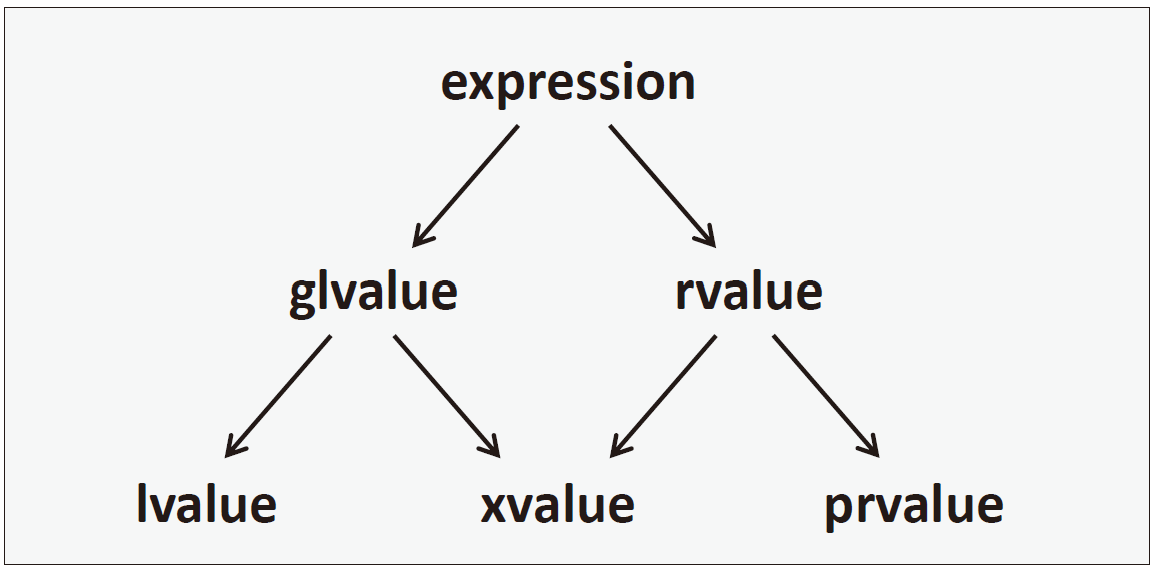
\includegraphics[width=1.0\textwidth]{content/1/chapter8/images/1}
\end{center}

有以下主要类别:\par

\begin{itemize}
	\item lvalue (“定位值”)
	\item prvalue (“纯可读值”)
	\item xvalue (“过期值”)
\end{itemize}

综合类别为:\par

\begin{itemize}
	\item glvalue (“广义lvalue”)作为“左lvalue或xvalue”的常用术语
	\item rvalue作为“xvalue或prvalue”的常用术语
\end{itemize}

\hspace*{\fill} \par %插入空行
\textbf{基本表达式的值分类}\par

lvalue的例子有:\par

\begin{itemize}
	\item 仅为变量、函数或数据成员(除右值的普通值成员外)的名称的表达式
	\item 只是字符串字面量的表达式(例如,"hello")
	\item 如果函数声明返回左值引用,则返回函数的值(返回类型type \&)
	\item 任何对函数的引用,即使标记为\textit{std::move()}(参见下面)
	\item 内置的一元操作符*的结果(即,对原始指针进行解引用所产生的结果)
\end{itemize}

prvalue的例子有:\par

\begin{itemize}
	\item 由非字符串字面量的内置字面量组成的表达式(例如,42、true或nullptr)
	\item 如果函数声明为按值返回,则按类型返回值(返回类型为Type)。
	\item 内置的一元操作符\&的结果(即,获取表达式的地址所产生的结果)
	\item Lambda表达式
\end{itemize}

xvalues的示例如下:\par

\begin{itemize}
	\item 用\textit{std::move()}标记对象的结果
	\item 对对象类型(不是函数类型)的rvalue引用的强制转换
	\item 函数声明返回rvalue引用(返回类型type \&\&)
	\item 右值的非静态值成员(见下面)
\end{itemize}

例如:\par

\begin{lstlisting}[caption={}]
class X {
};

X v;
const X c;

f(v); // passes a modifiable lvalue
f(c); // passes a non-modifiable lvalue
f(X()); // passes a prvalue (old syntax of creating a temporary)
f(X{}); // passes a prvalue (new syntax of creating a temporary)
f(std::move(v)); // passes an xvalue
\end{lstlisting}

说些经验法则:\par

\begin{itemize}
	\item 所有用作表达式的名称都是lvalue。
	\item 所有用作表达式的字符串字面值都是lvalue。
	\item 所有非字符串字面值(4.2、true或nullptr)都是prvalue。
	\item 所有没有名称的临时对象(特别是回的对象)都是prvalues。
	\item 所有标记为\textit{std::move()}的对象,及其值成员都是xvalues。
\end{itemize}

严格来说,glvalues、prvalues和xvalues是表达式的术语,而不是值的术语(这意味着这些术语用词不当)。例如,变量本身不是lvalue,只有表示该变量为lvalue的表达式:\par

\begin{lstlisting}[caption={}]
int x = 3; // here, x is a variable, not an lvalue
int y = x; // here, x is an lvalue
\end{lstlisting}

第一个语句中,3是一个初始化变量x的prvalue(不是lvalue)。第二个语句中,x是一个lvalue(它的计算值指定了一个包含值3的对象)。lvalue x用作rvalue,它初始化变量y。\par

\hspace*{\fill} \par %插入空行
\textbf{8.1.3 C++17新加的值类别}

C++17具有相同的值类别,图8.2中描述了值类别的语义。\par

现在解释值类别有两种主要的表达方式:\par

\begin{itemize}
	\item glvalues: 用于长生命周期对象或函数位置的表达式
	\item prvalues: 用于短生命周期对象的初始化表达式
\end{itemize}

然后,xvalue是表示不再需要其资源/值的(长期存在的)对象。\par

\hspace*{\fill} \par %插入空行
图8.2 C++17新加的值类别\par

\begin{center}
	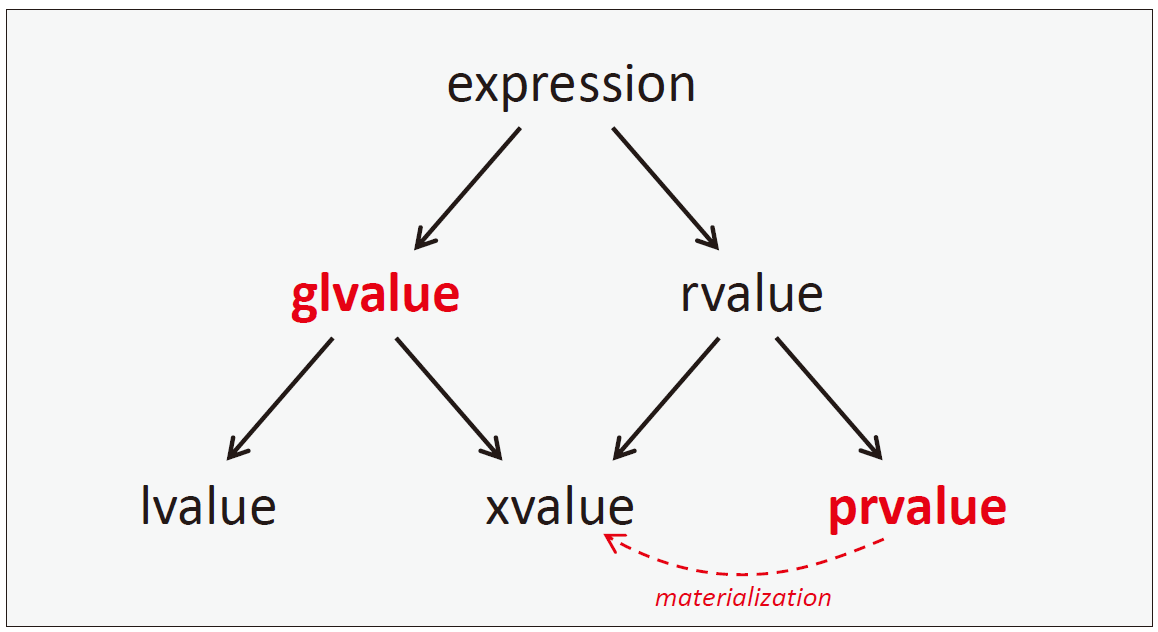
\includegraphics[width=1.0\textwidth]{content/1/chapter8/images/2}
\end{center}

\hspace*{\fill} \par %插入空行
\textbf{通过值传递prvalues}

有了这个更改,即使没有定义有效的副本和有效的移动构造函数,现在也可以将prvalue作为未命名的初始值按值传递:\par

\begin{lstlisting}[caption={}]
class C {
	public:
	C( ... );
	C(const C&) = delete; // this class is neither copyable ...
	C(C&&) = delete; // ... nor movable
};

C createC() {
	return C{ ... }; // Always creates a conceptual temporary prior to C++17.
} // In C++17, no temporary object is created at this point.

void takeC(C val) {
	...
}

auto n = createC(); // OK since C++17 (error prior to C++17)

takeC(createC()); // OK since C++17 (error prior to C++17)
\end{lstlisting}

C++17之前,如果没有复制或移动支持,传递prvalue(例如:\textit{createC()}的创建和初始化返回值)是不可能的。但是,从C++17开始,只要是不需要有地址的对象,就可以按值传递prvalues。\par

\hspace*{\fill} \par %插入空行
\textbf{具象化}

C++17随后引入了一个新术语,称为具象化(未命名的临时对象),此时prvalue变成了临时对象。因此,临时物化转换是prvalue到xvalue转换(通常是隐式的)。\par

需要glvalue(左值或xvalue)的地方使用prvalue,就会创建临时对象,并使用该prvalue初始化(记住,prvalue主要是“初始化值”),并且该prvalue会指定临时对象的xvalue。因此,在上面的例子中:\par

\begin{lstlisting}[caption={}]
void f(const X& p); // accepts an expression of any value category but expects a glvalue

f(X{}); // creates a temporary prvalue and passes it materialized as an xvalue
\end{lstlisting}

因为本例中的\textit{f()}有一个引用形参,所以需要一个glvalue参数。然而,表达式X\{\}是prvalue。因此,“临时具象化”的规则开始起作用,表达式X\{\}被“转换”为xvalue,该xvalue指定使用默认构造函数初始化的临时对象。\par

请注意,具象化并不意味着我们创建新的/不同的对象。左值引用\textit{p}仍然绑定到xvalue和prvalue,尽管后者现在会涉及到向xvalue的转换。\par






